\documentclass[11pt]{article}

\usepackage[margin=1in]{geometry}
\usepackage{graphicx}
\usepackage{float}
\usepackage{caption}
\usepackage{amsmath}
\usepackage{hyperref}
\usepackage{xurl}

\captionsetup{font=small, labelfont=bf}
\setlength{\textfloatsep}{10pt}
\setlength{\floatsep}{8pt}

\title{COMP 396 Mine Production and Inventory Control Project Report}
\author{Alexander Halimi}
\date{\today}

\begin{document}

\maketitle

\begin{abstract}
This report presents a COMP 396 project on mine production and ore stockpile inventory control, completed in collaboration with Professor Alessandro Navarra. The project began with Arena-based modeling and evolved into a modular Python simulation framework that loads model expressions directly from Excel and supports Bayesian optimization of control variables. The report summarizes the project motivation, technical background, implementation contributions, relationship to prior work, and future directions.
\end{abstract}

\section*{Collaboration Acknowledgment}
This project was conducted in collaboration with Professor Alessandro Navarra. His Arena model design, project direction, and technical feedback were central to both the simulator implementation and the optimization framework.

\section{Introduction}
This project evolved from introductory Arena exercises into a complete Python-based simulation and optimization workflow for a mine production and ore stockpile inventory control system. The initial objective was to understand the Arena logic in sufficient depth to reproduce it faithfully in code; the second objective was to extend that foundation by tuning control variables from repeated simulation results.

A major advantage was that Professor Alessandro Navarra's Arena model already behaved similarly to a traditional program. This made it possible to map key model components to separate Python modules without compromising the original logic.

This objective has clear practical importance: production policy choices directly affect throughput, shutdown exposure, and stockout risk. Even small improvements in control parameters can translate into meaningful gains in ore processed per unit time, better utilization of operating modes, and reduced performance loss from poorly timed transitions. In short, optimizing control settings is not only a modeling exercise; it is central to improving operational efficiency in a constrained mine-production environment.

\section{Background}
To understand the final implementation, the reader needs background on both the Arena progression and the simulation-control setting used in the mine model. The system combines production dynamics, mode switching, and ore stockpile thresholds, with performance measured primarily through throughput while monitoring stock behavior and shutdown impact.

\subsection{Problem Formulation}
At a high level, the project addresses a simulation-based control problem. Let the simulator state at time $t$ be denoted by
\[
s_t = \big(\mathbf{L}_t, \mathbf{T}_t, \mathbf{N}_t, \mathbf{C}_t, r_t\big),
\]
where $\mathbf{L}_t$ are continuous levels (including ore extraction and stock levels), $\mathbf{T}_t$ are timers that measure time spent in operational modes, $\mathbf{N}_t$ are discretely dynamical numerical variables, $\mathbf{C}_t$ are categorical variables, and $r_t$ is the active rate-configuration index.

State evolution is event-driven: the simulator computes the next threshold crossing, advances time to that event, updates all levels and timers according to active rates, executes assignment logic, and then updates the rate configuration. This repeats until the terminating condition in the Arena expression set evaluates to true.

The control task is to choose policy variables that produce favorable long-run behavior. In the current implementation, the principal optimization target is throughput, while preserving stock-control behavior defined in the original Arena logic.

\subsection{Why Simulation-Based Optimization Is Needed}
In this setting, the objective function is not available in closed form. It is generated by running the full simulator, which is computationally expensive and may contain stochastic effects due to randomized inputs. This rules out standard analytic optimization methods and motivates a black-box optimization approach. Bayesian optimization is a natural fit because it can use relatively few simulator calls while still exploring the policy space in a structured way.

\subsection{Performance Metric}
The core performance metric used in this project is throughput. If $E$ is cumulative ore extracted, $E_{\text{warmup}}$ is ore extracted during warm-up, and $T_{\text{active}}$ is total non-shutdown operating time, then throughput is computed as
\[
\text{Throughput} = \frac{E - E_{\text{warmup}}}{T_{\text{active}}}.
\]
This definition reflects production efficiency after warm-up bias is removed. Additional timer-based quantities are tracked to measure how much time the system spends in each operating mode.

\section{Semester Progression in Arena}

Throughout the semester, the Arena model evolved through three distinct phases, each building on the previous to increase complexity and introduce new modeling techniques. This section summarizes each phase and its role in informing the eventual Python implementation.

\subsection{Getting Familiar with Arena (Queue Network)}
At the beginning, I focused on mastering Arena fundamentals. We built a basic queue network to understand entity movement, delays, event logic, and state evolution over time.

\begin{figure}[H]
\centering
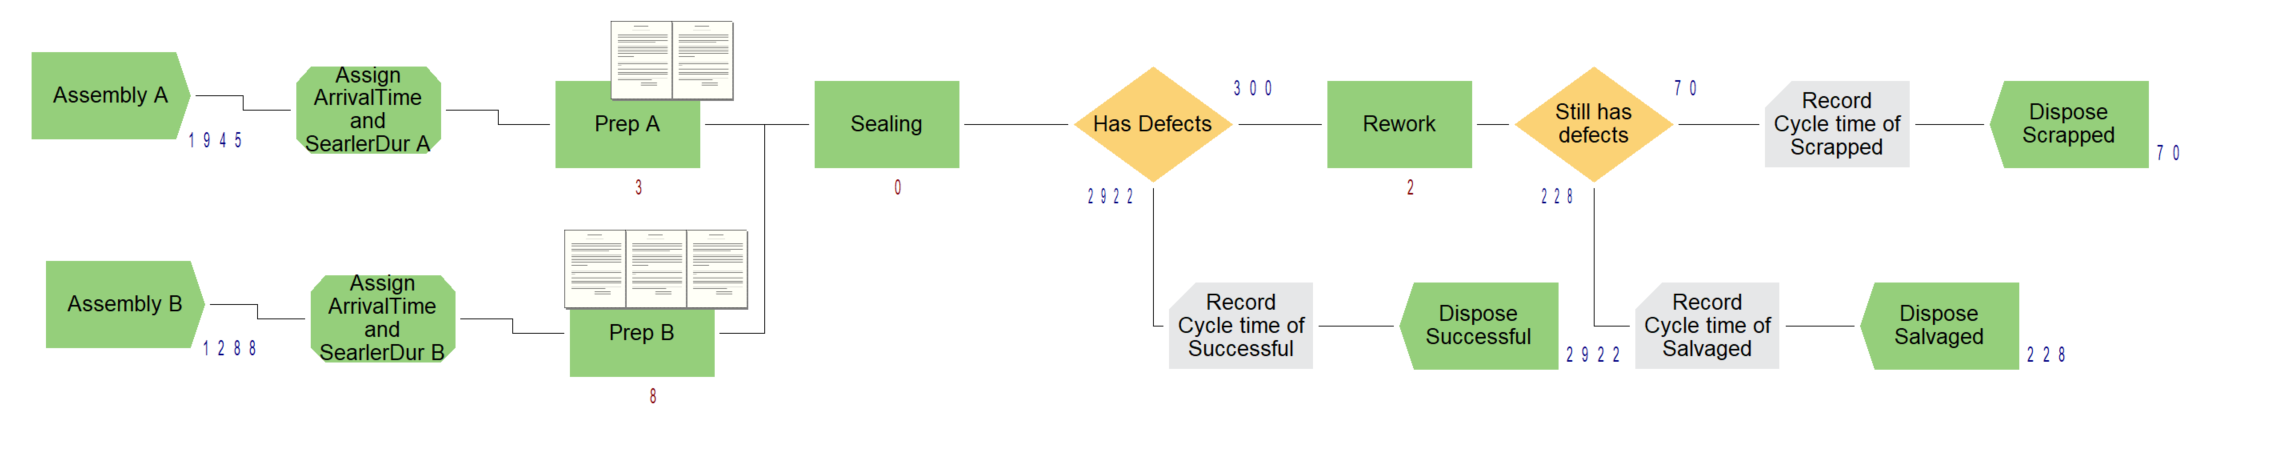
\includegraphics[width=0.82\linewidth]{images/Model1.png}
\caption{Arena Part 1: Basic queue network model.}
\label{fig:arena-part1-queue}
\end{figure}

\subsection{Simple Inventory Model with VBA}
The next stage was a simple inventory model with VBA integration. This was the point where VBA was formally introduced into the workflow. At this stage, stockout behavior and order volume were treated as control variables, which naturally motivated parameter tuning based on observed system outputs.

\begin{figure}[H]
\centering
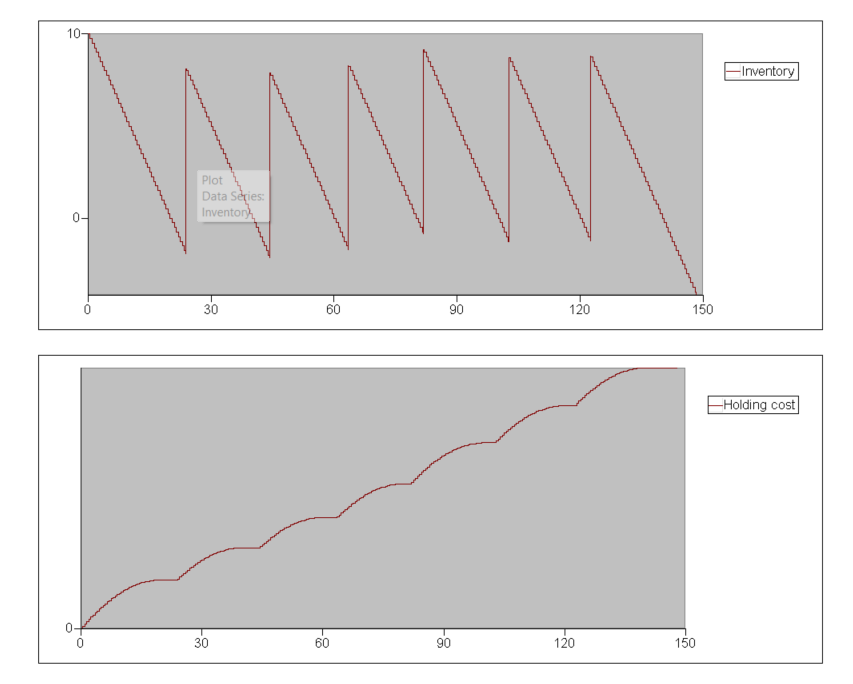
\includegraphics[width=0.49\linewidth]{images/Model2_1.png}\hfill
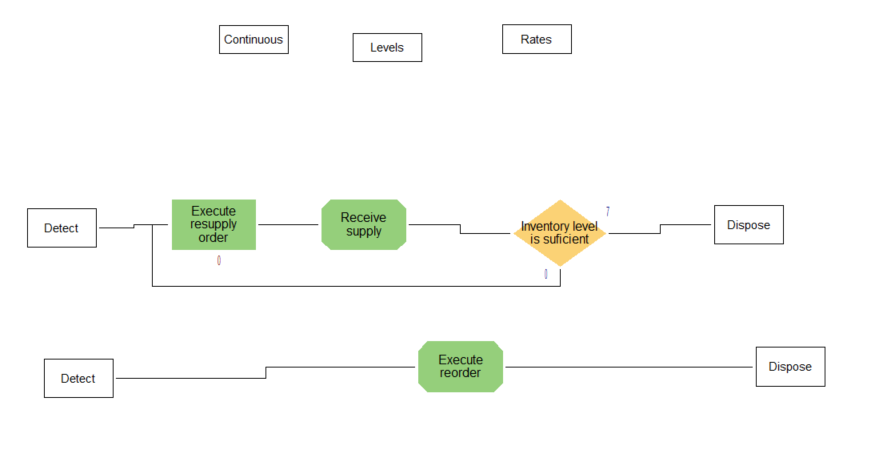
\includegraphics[width=0.49\linewidth]{images/Model2_2.png}
\caption{Arena Part 2: Inventory model with VBA and control variables.}
\label{fig:arena-part2-inventory-vba}
\end{figure}

\subsection{Mine Factory Production and Stockpile Control Model}
The third Arena phase was a larger mine-factory model that combined production flow with ore stockpile control. This version retained and extended the VBA-assisted logic from the previous phase while introducing substantially more complexity in threshold management, state updates, and operating modes. The program-like structure of Professor Alessandro Navarra's Arena model directly informed the Python architecture used in this project.

\begin{figure}[H]
\centering
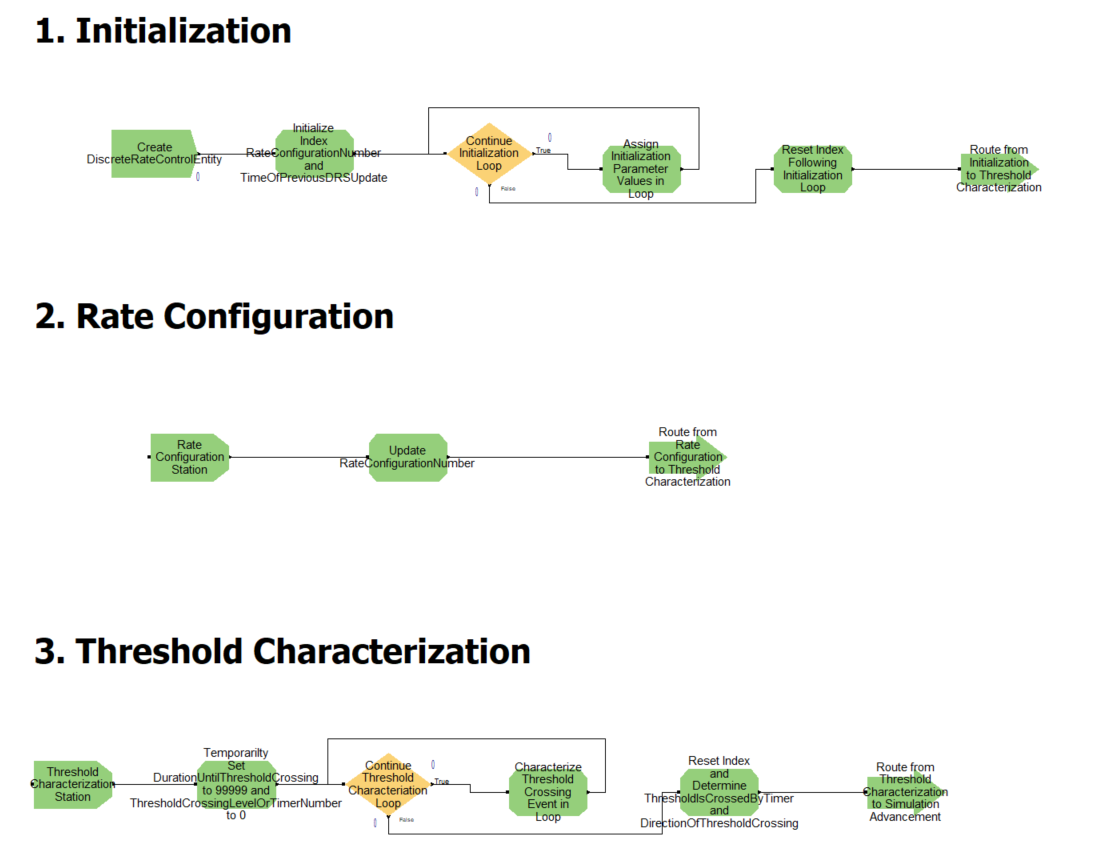
\includegraphics[width=0.49\linewidth]{images/Model3_1.png}\hfill
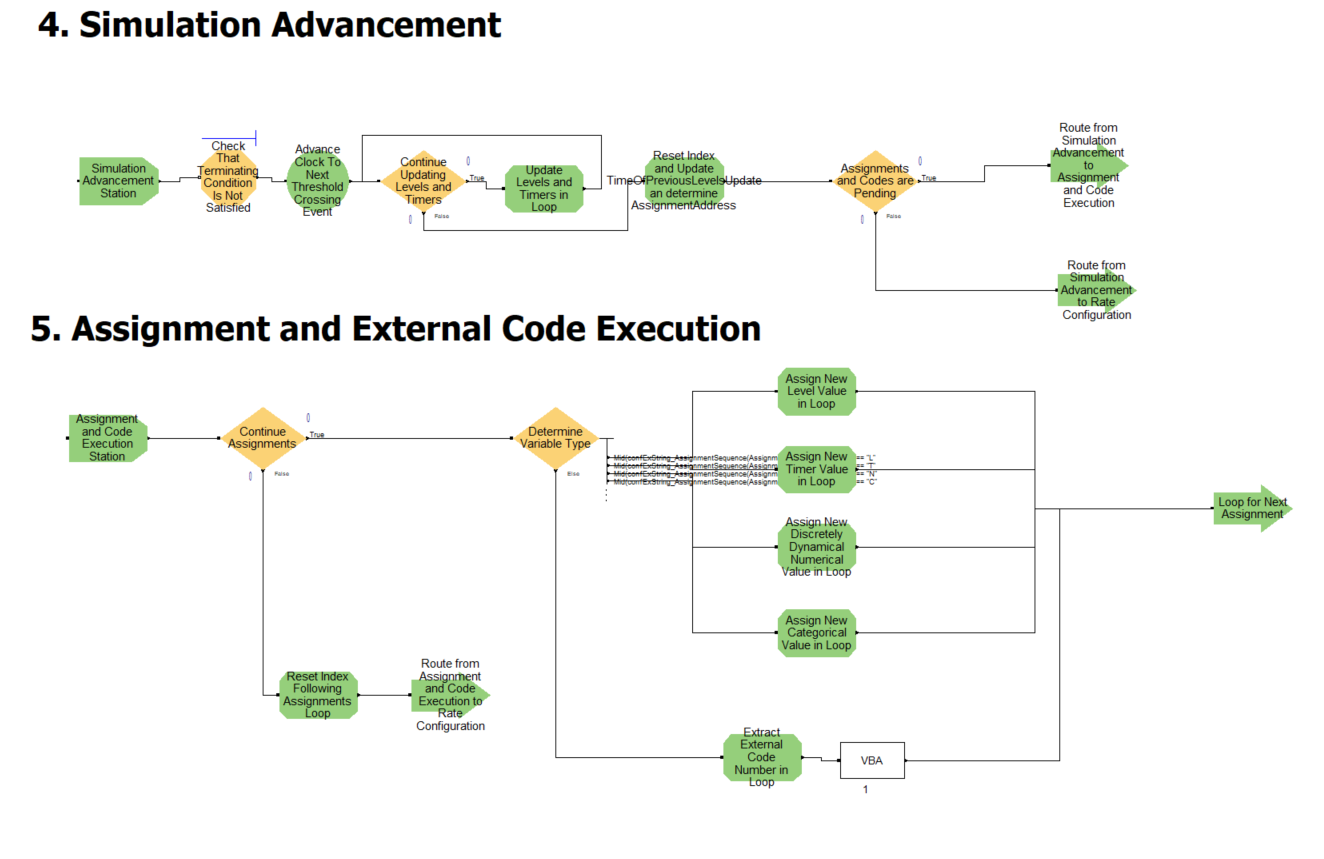
\includegraphics[width=0.49\linewidth]{images/Model3_2.png}
\caption{Arena Part 3: Mine factory production and stockpile control model.}
\label{fig:arena-part3-mine}
\end{figure}

\section{Contribution: Python Implementation and Optimization}
The implementation strategy was to avoid manually copying model logic and instead load Arena configuration expressions directly from the provided Excel file. To support this, I wrote a parser and organized the codebase into separate modules for each major simulation component.

\subsection{Architecture Choices}
The project is divided into dedicated modules for initialization, threshold characterization, simulation advancement, assignment execution, rate-configuration updates, output statistics, plotting, and optimization. This modular design improved maintainability and made debugging more tractable as the implementation grew.

Custom expression handling was required because Arena syntax differs from Python syntax. I implemented a translation layer for operators (for example, replacing \texttt{\&\&}, \texttt{||}, and \texttt{<>}) and used a controlled evaluator to execute Arena-style expressions in Python.

\subsection{Configuration from Excel Instead of Manual Copying}
A key design decision was to load configuration expressions directly from the Excel sheet provided by Professor Alessandro Navarra into Python dataclasses. This preserved consistency with the Arena model and reduced transcription errors from manual rewriting.

\subsection{Implementation Challenge: Indexing and Tooling Decisions}
One early source of errors came from a structural mismatch between Arena and Python indexing conventions. Arena expressions and model logic often assume 1-indexed arrays, while Python uses 0-indexed arrays by default. During initial implementation, this difference introduced indexing bugs in expression evaluation and state updates, especially when mapping labels and matrix-like configuration values into Python lists.

To address this, I introduced explicit index-handling utilities in key evaluation paths and progressively aligned indexing behavior across the simulation pipeline. This was an important stabilization step and reduced hard-to-trace logic errors.

I also initially considered implementing the optimization workflow in Java, mainly for two reasons: Java performance and my prior comfort with Java concurrency. I eventually decided to keep the optimization implementation fully in Python to reduce development complexity and keep the workflow in a single language.

That said, a strong future optimization remains available: using a Java orchestration layer to run multiple simulator instances on separate threads. Since many simulation runs are independent, concurrent execution could provide substantial speedups for replication-heavy experiments. I did not prioritize this path in the final implementation to keep development simpler, but it is a practical and potentially high-impact performance improvement.

\subsection{Simulation Flow in Brief}
At runtime, the simulator initializes levels and timers from Excel expressions, identifies the next threshold crossing, and advances time to that event. It then updates levels and timers using the active rate configuration, executes the assignment sequence associated with the crossing, updates rate configuration when required, and repeats this loop until the termination condition is satisfied. The final stage computes output statistics and generates plots for mode behavior and ore levels.

\subsection{Implementation Design Decisions and Trade-Offs}
Several design decisions had a strong impact on the final system. First, expression strings were kept close to the Arena source rather than translated into a completely new domain model. This improved traceability when debugging differences between Arena and Python, but it also required careful expression evaluation and environment construction at runtime.

Second, the implementation favored explicit modularity over compactness. Splitting the code into narrowly focused files introduced more moving parts, but made it easier to isolate failures, inspect intermediate state updates, and test individual parts of the event loop. This was especially useful once optimization was introduced, because many repeated simulator runs amplified any hidden consistency bug.

Third, the implementation deliberately prioritized traceability over aggressive optimization in the core simulator code. This made debugging and validation easier during development, even when it meant accepting short-term performance trade-offs.

\begin{figure}[H]
\centering
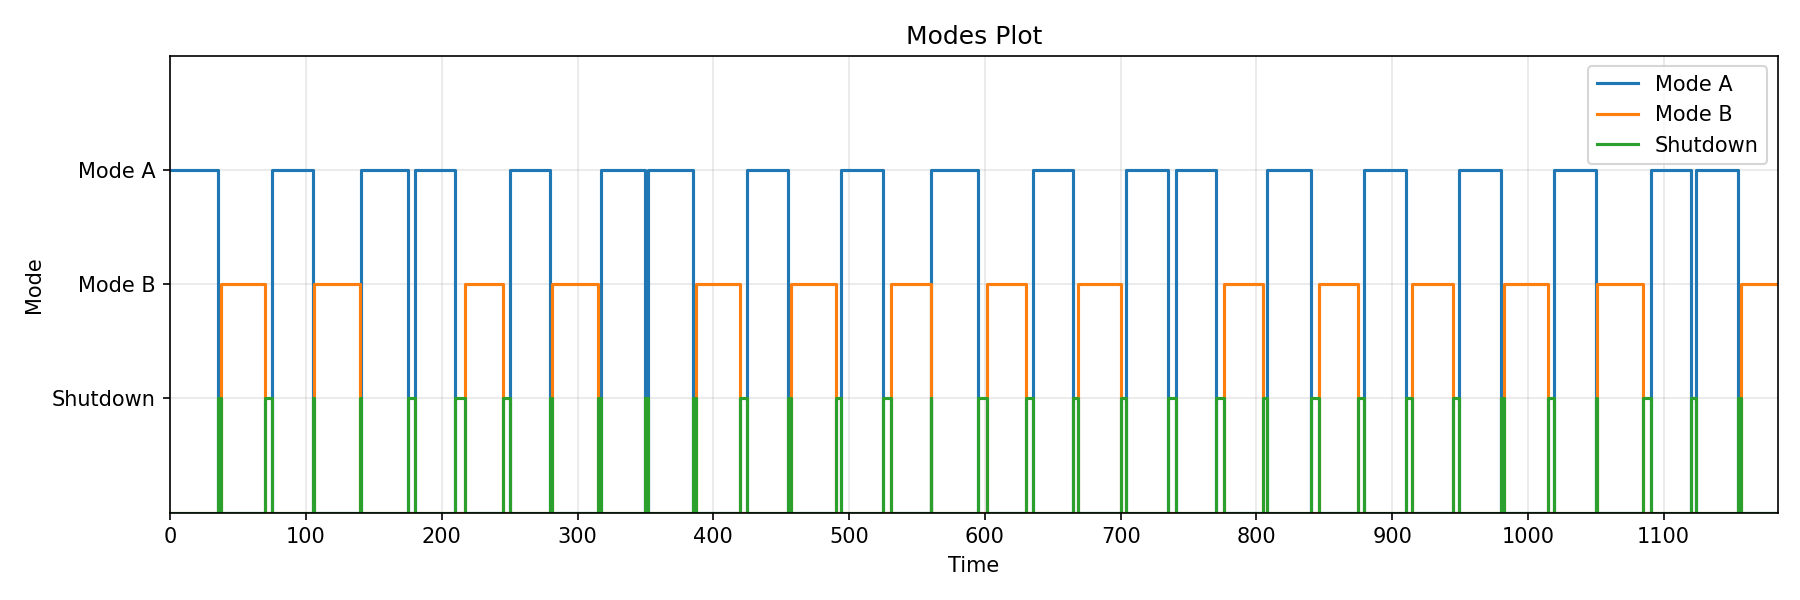
\includegraphics[width=0.82\linewidth]{images/Python_sim_modes_plot.png}
\caption{Python simulator output: operating mode evolution over time.}
\label{fig:software-architecture}
\end{figure}

\section{From Parallel Runs to Optimization Focus}
My initial extension was a Java-based parallel runner to execute many simulation replications concurrently and improve statistical reliability more efficiently. This was implemented by launching multiple Python simulation processes and aggregating their outputs.

That Java-based multithreading produced a major wall-clock speedup, but the parallel implementation itself was straightforward enough that I did not want to spend the project mainly on runtime reduction. I moved to optimization instead because reducing average simulation time felt too incremental on its own, while tuning the control variables had a much larger impact on the actual system behavior and final outpu

\subsection{Observed Runtime Comparison: Java Concurrency vs Python Sequential}
To document the implementation-performance impact, I recorded average runtime results for Java and Python execution paths. The Java result was measured using 5 threads over 15 occurrences, while the Python sequential result was measured over 10 occurrences.

\begin{figure}[H]
\centering
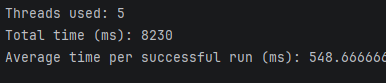
\includegraphics[width=0.49\linewidth]{images/Java_performance.png}\hfill

\includegraphics[width=0.49\linewidth]{images/Python_sequential_avg.png}
\caption{Average runtime comparison. Left: Java concurrent execution (5 threads, 15 occurrences). Right: Python sequential execution (10 occurrences).}
\label{fig:java-python-speed-comparison}
\end{figure}

These runtime comparisons showed a clear improvement when Java multithreading was used. Since that speedup was already achieved, I chose not to pursue that path further and instead redirected effort toward something more complex and higher-impact: optimization of the control variables.


\begin{figure}[H]
\centering
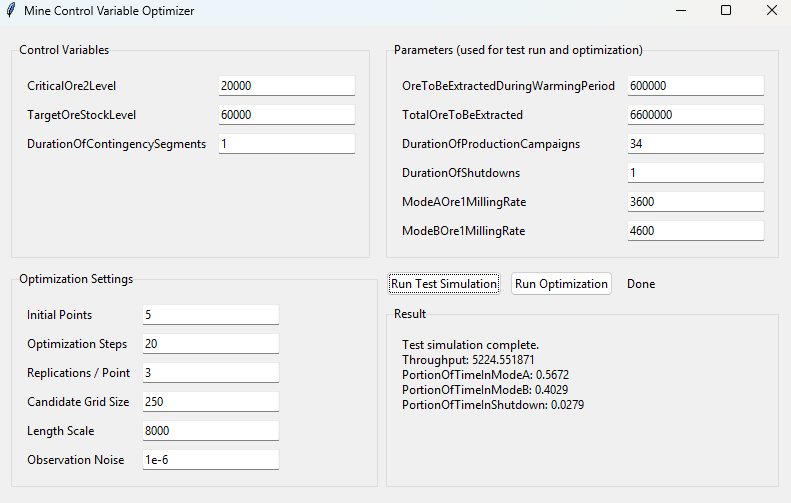
\includegraphics[width=0.49\linewidth]{images/Python_sim_Run_single_test.png}\hfill
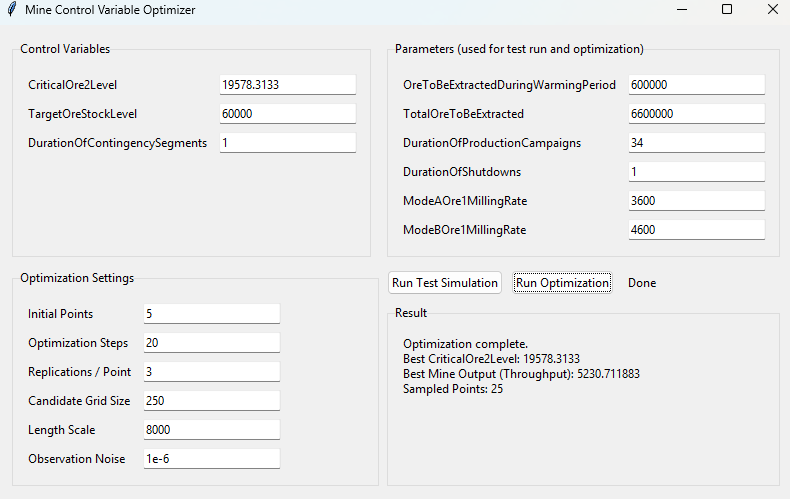
\includegraphics[width=0.49\linewidth]{images/Python_sim_Run_optimization.png}

\vspace{0.5em}

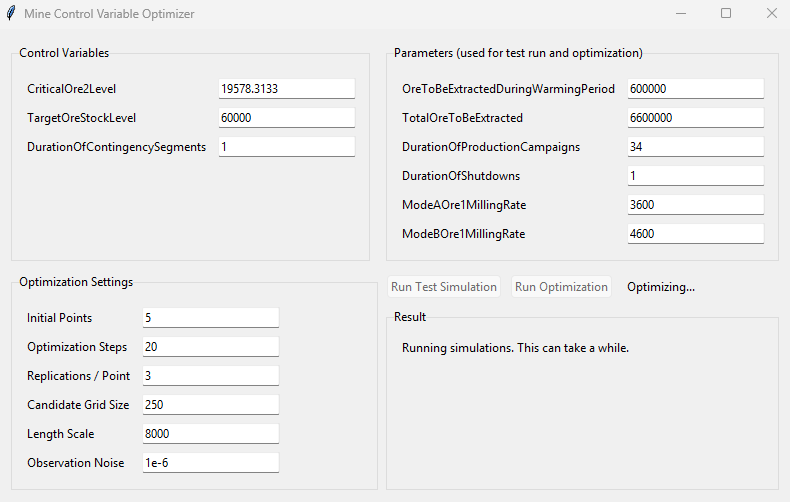
\includegraphics[width=0.72\linewidth]{images/Python_sim_Optimization_in_progress.png}
\caption{Python UI workflow: single test run, optimization launch, and optimization in progress.}
\label{fig:python-ui-workflow}
\end{figure}


\subsection{Optimization Method and Rationale}
The optimization method used was Bayesian optimization, implemented with a GP-style predictive model and expected-improvement-style candidate scoring, to tune key control variables, particularly the critical ore stock threshold.

\subsection{Bayesian Optimization Procedure Used in This Project}
The optimization loop follows four recurring steps:
\begin{enumerate}
	\item Sample initial candidate control values over a bounded interval.
	\item Evaluate each candidate by running multiple simulator replications and averaging the objective.
	\item Compute candidate scores from previously observed samples.
	\item Select the next candidate by maximizing an acquisition score, then repeat.
\end{enumerate}

In this project, the objective is formulated as minimization of negative throughput, so maximizing throughput is equivalent to minimizing
\[
f(x) = -\text{Throughput}(x).
\]
For each candidate $x$, the estimate is
\[
\hat f(x) = \frac{1}{R}\sum_{i=1}^{R} f_i(x),
\]
where $R$ is the number of replications.

Given observed data $\mathcal{D} = \{(x_j, y_j)\}_{j=1}^{n}$, the predictive model produces a mean estimate $\mu(x)$ for each candidate. The acquisition stage uses this estimate to score candidates against the current best observed objective, which reduces wasteful simulator calls compared with dense grid evaluation.

\subsection{Acquisition Intuition and Practical Implications}
The expected-improvement-style acquisition can be interpreted as asking: ``How much better than the current best result could this candidate be?'' In practice, this produced stable search behavior in this project and improved sample efficiency compared with naïve sweeps.

From an engineering perspective, this balance was important because simulator runs were expensive enough that purely exploratory search would be slow, while purely exploitative search risked premature convergence.

\subsection{Why Bayesian Optimization Instead of Simpler Regression}
Bayesian optimization was selected because each simulator evaluation is relatively expensive, so the method must learn effectively from a limited number of trials. The mine system is nonlinear and includes interacting variables, making linear regression a weak fit for this tuning problem. The predictive model guides where to sample next by balancing exploration and exploitation. This approach was also informed by prior exposure in COMP 551 and matched the structure of this simulation-driven setting.

\subsection{Learning Process and References}
One challenge was finding references that were both mathematically rigorous and implementation-oriented. The most useful materials were the Cornell notes in the bibliography \cite{cornell4780note15,cornell4787lec16,cornell4787lec17}. These helped connect theoretical intuition with practical optimization decisions used in this project.

\subsection{Optimization Objective (Current Form)}
The current implementation maximizes throughput by minimizing its negative value over selected control settings:
\[
\min_{x \in [x_{\min}, x_{\max}]} f(x), \quad f(x) = -\text{Throughput}(x)
\]
where $x$ is a control variable (e.g., critical ore level) and throughput is measured from replicated simulation runs.

In practical terms, the optimization is currently centered on production performance while preserving stock-level control behavior encoded in the simulator.

\subsection{Experimental Protocol Used for Optimization Runs}
To reduce variance in optimization outcomes, each candidate configuration was evaluated with multiple replications under different random seeds. Candidate bounds were constrained by control-variable meaning (for example, critical stock thresholds constrained by target stock level). The workflow used in practice was:
\begin{enumerate}
	\item Verify baseline behavior with a single-run test.
	\item Launch optimization from the UI with selected replication count and step budget.
	\item Record the best control variable and objective value returned by the optimizer.
	\item Compare candidate behavior against baseline to detect unstable policy choices.
\end{enumerate}

This protocol reflects the actual optimization pipeline, which computes the best variable using objective evaluations only.

\begin{figure}[H]
\centering
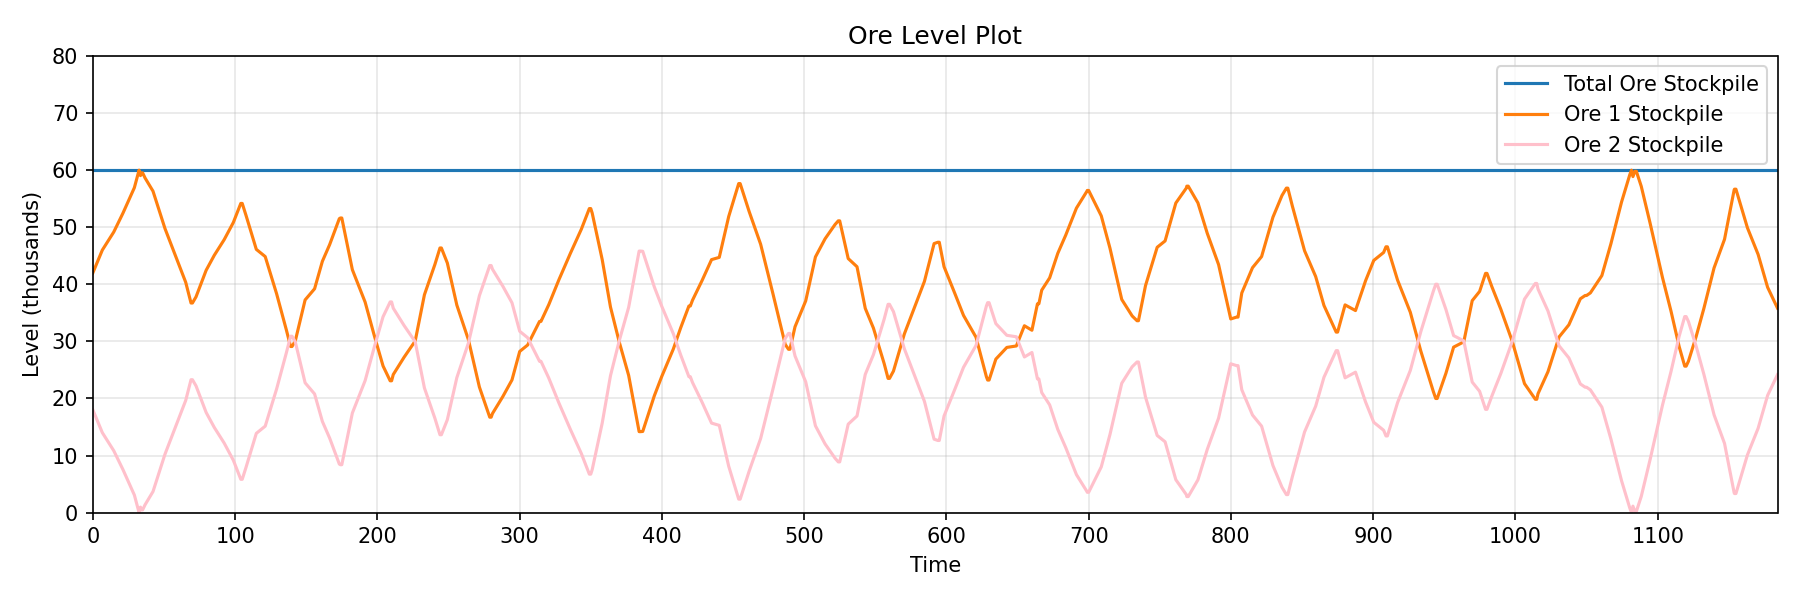
\includegraphics[width=0.82\linewidth]{images/Python_sim_ore_level_plot.png}
\caption{Python simulator output file: ore stock levels over time. During optimization runs, plot generation is disabled to reduce overhead and improve runtime performance.}
\label{fig:optimization-ui}
\end{figure}

\section{Related Work}
% TODO: check Navarra docs for any additional related-work references or wording.
This project is related to two main areas of work: simulation-based control and Bayesian optimization. In simulation-based control, the system is evaluated repeatedly and control settings are tuned by comparing outcomes across runs. That is the basic pattern used in this DRS project, where the simulator itself is the only practical way to measure the effect of a control choice.

For the optimization side, the implementation follows the standard Bayesian optimization idea of using previous evaluations to choose the next candidate more intelligently than a brute-force sweep. The Cornell lecture notes in the bibliography were useful as background for the terminology and practical intuition behind the method \cite{cornell4780note15,cornell4787lec16,cornell4787lec17}.

The key point for this report is that the project combines these two ideas in one implementation: a DRS simulator for mine production and stockpile control, and a Bayesian search procedure that uses repeated simulation results to tune control variables.

\section{Discussion: What Worked and What Did Not}
The current implementation has several limitations. The simulation outputs are aligned with the Arena baseline for the tested workflow. The optimization layer is currently narrow and focuses on a limited subset of control variables. In addition, a formal unit-testing suite is still absent, and the expression translation covers core syntax but not every Arena construct.

At the same time, several components worked well in practice. The modular architecture made iterative development manageable, particularly when debugging threshold characterization and assignment execution. Direct loading from Excel was also successful: once parsing was stable, it substantially reduced manual synchronization errors between the Arena model and Python code.

Another successful outcome was the transition from code-based optimization to a usable UI workflow. The optimization engine was implemented first, and the UI was added afterward to improve experimentation speed and run-status visibility.

\subsection{Threats to Validity}
There are three main threats to validity in the current results. First, model validity depends on faithful expression translation and environment construction; any mismatch can propagate through the event loop. Second, stochastic variability means that insufficient replications may overstate gains for a candidate configuration. Third, the current objective does not explicitly price costs associated with mode transitions; a more detailed objective could account for transition penalties and other operational economics.

\section{Conclusions and Future Work}
This project began with foundational Arena modeling and matured into a modular Python simulator for mine production and ore stockpile control, complemented by an optimization workflow for control-variable tuning. Its primary contribution is the direct expression-driven architecture loaded from the provided Excel model, together with a shift from manual parameter adjustment to algorithmic search.

Several strong directions remain for future work. The most immediate is extending from single-variable tuning to joint optimization over multiple control variables, followed by objective formulations that combine throughput, stockout behavior, shutdown impact, and transition-related operating costs. From a computational perspective, combining parallel replications with optimization should improve statistical confidence while reducing runtime. Queueing-theory abstractions may also provide clearer analytical insight into bottlenecks. Performance profiling is needed as well, particularly around plotting and file-I/O overhead.

Another practical extension would be to keep the optimization logic in Python but move execution to Java, using a thread pool to dispatch program setups and \texttt{Future} objects to collect results asynchronously. That would preserve the current search logic while giving the execution layer a more scalable runtime design.

A separate next step is to formalize a benchmarking suite with fixed seeds, standardized scenario files, and reporting templates. This would make future comparisons reproducible and would support supervisor review by clearly separating algorithmic improvements from random variation.

\appendix

\section{Implementation Notes}
The implementation is organized around modular Python files for state initialization, threshold characterization, simulation advancement, assignment execution, rate-configuration updates, output statistics, and optimization. A separate Java utility was also implemented for concurrent replications.

The most implementation-sensitive modules are the expression evaluator, environment builder, threshold characterization logic, and assignment execution pipeline. Together, these determine whether Arena semantics are preserved at runtime. In development, most debugging effort concentrated on these modules, since small expression or indexing mismatches can induce large downstream behavioral differences.

\section{Reproducibility}
Typical execution workflow:
\begin{itemize}
	\item Run simulator: \texttt{python DRS\_Simulator.py}
	\item Run optimization: \texttt{python bayesian\_stockout\_regression.py}
	\item Run UI: \texttt{python control\_optimizer\_ui.py}
	\item Parallel runs: \texttt{java run\_concurrently <numRuns> <numThreads> [pythonCmd]}
\end{itemize}

For reproducible comparisons, it is recommended to keep replication count, optimization step budget, and control-variable bounds fixed across experiments, while varying only one design choice at a time. This makes observed differences easier to attribute and reduces ambiguity during supervisor review.

\begin{thebibliography}{9}

\bibitem{cornell4780note15}
Cornell CS4780.
\newblock \emph{Lecture 15: Gaussian Processes}.
\newblock Cornell University, 2017.
\newblock \url{https://www.cs.cornell.edu/courses/cs4780/2017sp/lectures/lecturenote15.html}.

\bibitem{cornell4787lec16}
Cornell CS4787.
\newblock \emph{Lecture 16: Gaussian Processes and Bayesian
Optimization}.
\newblock Cornell University, 2019.
\newblock \url{https://www.cs.cornell.edu/courses/cs4787/2019sp/notes/lecture16.pdf}.

\bibitem{cornell4787lec17}
Cornell CS4787.
\newblock \emph{Lecture 17: Bayesian Optimization II}.
\newblock Cornell University, 2019.
\newblock \url{https://www.cs.cornell.edu/courses/cs4787/2019sp/notes/lecture17.pdf}.

\end{thebibliography}

\end{document}
